% Figura da seção "Integração entre ARIMA e GARCH" (Cap. I).
% 13/11/2026, pedido do autor: substitui a proposta C (fluxo com a direção
% entrando no losango). Agora é o ciclo de um pregão, de cima para baixo, sem
% fórmula: série -> ARIMA (para que lado?) -> GARCH sobre os resíduos (com que
% risco?) -> losango do limiar. Se o GARCH vetar, o ciclo termina sem ordem; se
% não, a ordem sai no lado do ARIMA com o tamanho ajustado ao risco. Os dois
% caminhos chegam ao fim do pregão, e a seta da esquerda volta ao início no
% pregão seguinte (o robô decide uma vez por dia, na abertura; Cap. II,
% "Funcionamento do robô"). Versões anteriores em ia/relatorios/integracao-arima-garch/.
% Mesmo estilo das fig05/fig06.
\documentclass[11pt,border=2pt]{standalone}
\usepackage[T1]{fontenc}
\usepackage[utf8]{inputenc}
\usepackage{mathptmx}
\usepackage{tikz}
\usetikzlibrary{arrows.meta,positioning,calc,shapes.geometric}
\tikzset{
  seta/.style={-{Stealth[length=2.2mm]}, semithick},
  caixa/.style={rectangle, draw, semithick, fill=gray!10, rounded corners=2pt,
                align=center, minimum width=52mm, minimum height=10mm, font=\small},
  extremo/.style={rectangle, draw, semithick, fill=white, rounded corners=4mm,
                  align=center, minimum width=34mm, minimum height=8mm, font=\small},
  dado/.style={trapezium, trapezium left angle=75, trapezium right angle=105, draw,
               semithick, fill=white, align=center, minimum height=8mm, font=\small,
               trapezium stretches body},
  decisao/.style={diamond, draw, semithick, fill=white, aspect=2.4, align=center,
                  inner sep=1pt, font=\small},
  pergunta/.style={font=\small\itshape, align=left},
  pequeno/.style={font=\footnotesize, align=center},
}
\begin{document}
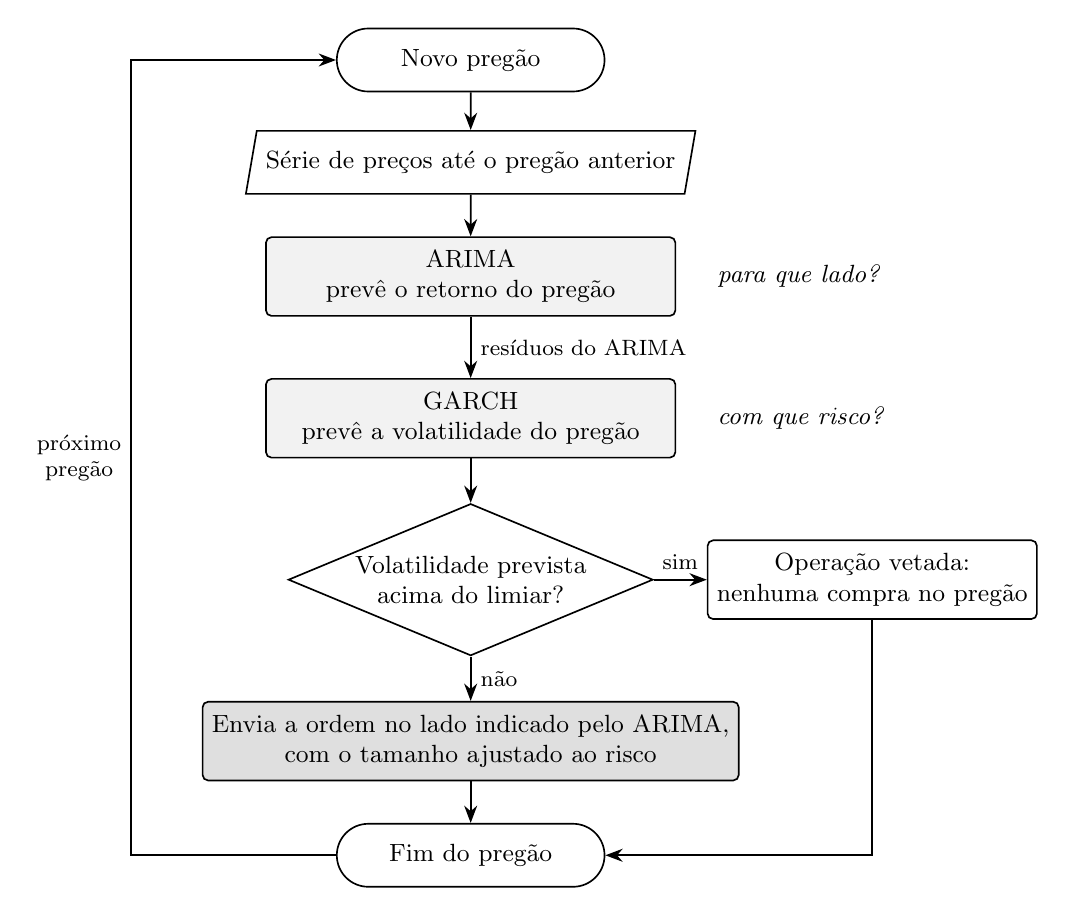
\begin{tikzpicture}
  \node[extremo] (ini) at (0,0) {Novo pregão};
  \node[dado] (serie) at (0,-1.3) {Série de preços até o pregão anterior};
  \node[caixa] (arima) at (0,-2.75) {ARIMA\\prevê o retorno do pregão};
  \node[caixa] (garch) at (0,-4.55) {GARCH\\prevê a volatilidade do pregão};
  \node[decisao] (lim) at (0,-6.6) {Volatilidade prevista\\acima do limiar?};
  \node[caixa, minimum width=40mm, fill=white] (veto) at (5.1,-6.6)
    {Operação vetada:\\nenhuma compra no pregão};
  \node[caixa, fill=gray!25] (ordem) at (0,-8.65)
    {Envia a ordem no lado indicado pelo ARIMA,\\com o tamanho ajustado ao risco};
  \node[extremo] (fim) at (0,-10.1) {Fim do pregão};

  \draw[seta] (ini) -- (serie);
  \draw[seta] (serie) -- (arima);
  \draw[seta] (arima) -- node[right, pequeno]{resíduos do ARIMA} (garch);
  \draw[seta] (garch) -- (lim);
  \draw[seta] (lim) -- node[above, pequeno]{sim} (veto);
  \draw[seta] (lim) -- node[right, pequeno]{não} (ordem);
  \draw[seta] (ordem) -- (fim);
  \draw[seta] (veto.south) |- (fim.east);
  \draw[seta] (fim.west) -- ++(-2.6,0) |- node[pos=0.25, left, pequeno]{próximo\\pregão} (ini.west);

  \node[pergunta, anchor=west] at ([xshift=4mm]arima.east) {para que lado?};
  \node[pergunta, anchor=west] at ([xshift=4mm]garch.east) {com que risco?};
\end{tikzpicture}
\end{document}
